\section{Workflow DFA-IA : Les 4 Phases}

Cette section détaille le workflow complet de DesignPro AI, structuré en 4 phases distinctes qui orchestrent l'ensemble du processus de conception assistée par IA.

\subsection{Vue d'Ensemble du Workflow}

Le workflow DFA-IA transforme une idée de produit en un concept visuel évalué et techniquement validé en moins d'une minute. La figure \ref{fig:workflow_complete} illustre ce processus.

\begin{figure}[H]
\centering
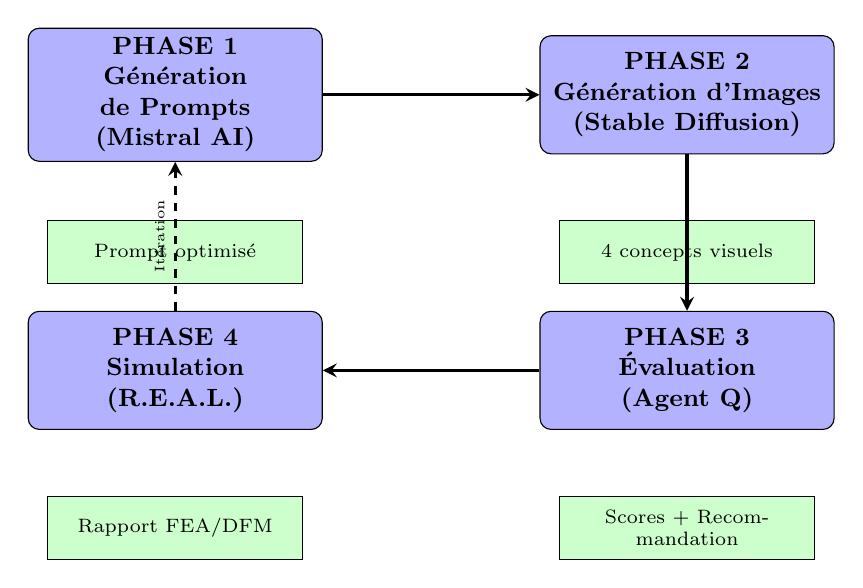
\begin{tikzpicture}[
    node distance=2.5cm,
    phase/.style={rectangle, draw, fill=blue!30, text width=3.5cm, text centered, rounded corners, minimum height=1.5cm, font=\small\bfseries},
    output/.style={rectangle, draw, fill=green!20, text width=3cm, text centered, minimum height=0.8cm, font=\scriptsize},
    arrow/.style={->, >=stealth, very thick}
]
    \node[phase] (p1) {PHASE 1\\Génération de Prompts\\(Mistral AI)};
    \node[phase, right of=p1, xshift=4cm] (p2) {PHASE 2\\Génération d'Images\\(Stable Diffusion)};
    \node[phase, below of=p2, yshift=-1cm] (p3) {PHASE 3\\Évaluation\\(Agent Q)};
    \node[phase, left of=p3, xshift=-4cm] (p4) {PHASE 4\\Simulation\\(R.E.A.L.)};
    
    \node[output, below of=p1, yshift=0.5cm] (o1) {Prompt optimisé};
    \node[output, below of=p2, yshift=0.5cm] (o2) {4 concepts visuels};
    \node[output, below of=p3, yshift=0.5cm] (o3) {Scores + Recommandation};
    \node[output, below of=p4, yshift=0.5cm] (o4) {Rapport FEA/DFM};
    
    \draw[arrow] (p1) -- (p2);
    \draw[arrow] (p2) -- (p3);
    \draw[arrow] (p3) -- (p4);
    \draw[arrow, dashed] (p4) -- (p1) node[midway, above, sloped, font=\tiny] {Itération};
\end{tikzpicture}
\caption{Workflow complet DFA-IA en 4 phases}
\label{fig:workflow_complete}
\end{figure}

\subsection{Phase 1 : Génération de Prompts Professionnels}

\subsubsection{Objectif}

Transformer une description de haut niveau en un prompt détaillé et optimisé pour les modèles de diffusion, intégrant les meilleures pratiques des méthodologies de design.

\subsubsection{Entrées Utilisateur}

L'utilisateur fournit 4 informations clés :

\begin{enumerate}[leftmargin=*]
    \item \textbf{Catégorie de produit} : Meuble, Électronique, Automobile, Outillage, Dispositif médical, etc.
    \item \textbf{Focus du design} : Ergonomie, Esthétique, Fonctionnalité, Durabilité, Innovation
    \item \textbf{Style visuel} : Minimaliste, Industriel, Futuriste, Organique, Rétro
    \item \textbf{Méthodologie} : TRIZ, Design Thinking, DFX, Value Engineering
\end{enumerate}

\subsubsection{Méthodologies de Design Intégrées}

\textbf{TRIZ (Theory of Inventive Problem Solving)} :
\begin{itemize}[leftmargin=*]
    \item Principes d'innovation (40 principes)
    \item Résolution de contradictions techniques
    \item Patterns d'évolution des systèmes
\end{itemize}

\textbf{Design Thinking} :
\begin{itemize}[leftmargin=*]
    \item Empathie utilisateur
    \item Idéation divergente
    \item Prototypage rapide
\end{itemize}

\textbf{DFX (Design for X)} :
\begin{itemize}[leftmargin=*]
    \item Design for Manufacturing (DFM)
    \item Design for Assembly (DFA)
    \item Design for Serviceability (DFS)
    \item Design for Sustainability (DFSust)
\end{itemize}

\textbf{Value Engineering} :
\begin{itemize}[leftmargin=*]
    \item Optimisation coût/fonction
    \item Analyse de la valeur
    \item Simplification
\end{itemize}

\subsubsection{Processus de Génération}

Mistral AI génère le prompt en suivant ce template structuré :

\begin{lstlisting}[caption=Template de génération de prompt]
Vous êtes un expert en design industriel spécialisé en [MÉTHODOLOGIE].

CONTEXTE:
- Catégorie: [CATÉGORIE]
- Focus: [FOCUS]
- Style: [STYLE]

MISSION:
Générez un prompt détaillé pour Stable Diffusion qui décrit un design de [CATÉGORIE] 
innovant, en appliquant les principes de [MÉTHODOLOGIE].

STRUCTURE DU PROMPT:
1. Description de la forme (géométrie, proportions)
2. Matériaux et textures
3. Couleurs et finitions
4. Contexte de rendu (éclairage, angle)
5. Style photographique

CONTRAINTES [MÉTHODOLOGIE]:
[Principes spécifiques à la méthodologie choisie]

Générez le prompt en 50-80 mots, optimisé pour Stable Diffusion.
\end{lstlisting}

\subsubsection{Exemple de Sortie}

\textbf{Entrée} :
\begin{itemize}[leftmargin=*]
    \item Catégorie : Meuble
    \item Focus : Ergonomie
    \item Style : Minimaliste
    \item Méthodologie : DFX
\end{itemize}

\textbf{Prompt généré} :
\begin{quote}
\textit{"A minimalist ergonomic office chair with flowing organic curves, featuring a breathable mesh backrest in charcoal gray, polished aluminum base with smooth-rolling casters, adjustable lumbar support visible through transparent side panels, designed for easy assembly with modular components, professional product photography, studio lighting, three-quarter view, high detail, 8k"}
\end{quote}

\subsection{Phase 2 : Génération d'Images de Design}

\subsubsection{Objectif}

Générer 4 concepts visuels distincts à partir du prompt optimisé, offrant une diversité d'exploration tout en maintenant la cohérence avec les spécifications.

\subsubsection{Modes de Génération}

\textbf{Mode 1 : Text-to-Image}

Génération pure à partir du prompt textuel :

\begin{lstlisting}[language=Python, caption=Génération text-to-image]
pipeline = StableDiffusionXLPipeline.from_pretrained(
    "stabilityai/stable-diffusion-xl-base-1.0",
    torch_dtype=torch.float16
)

images = pipeline(
    prompt=enhanced_prompt,
    negative_prompt="blurry, low quality, distorted",
    num_images_per_prompt=4,
    num_inference_steps=30,
    guidance_scale=7.5,
    width=1024,
    height=1024
).images
\end{lstlisting}

\textbf{Mode 2 : Sketch-to-Image}

Génération guidée par un croquis utilisateur :

\begin{lstlisting}[language=Python, caption=Génération sketch-to-image avec ControlNet]
# Prétraitement du sketch
canny_image = cv2.Canny(sketch, 100, 200)

# Génération avec ControlNet
controlnet = ControlNetModel.from_pretrained(
    "lllyasviel/sd-controlnet-canny"
)

pipeline = StableDiffusionControlNetPipeline.from_pretrained(
    "runwayml/stable-diffusion-v1-5",
    controlnet=controlnet
)

images = pipeline(
    prompt=enhanced_prompt,
    image=canny_image,
    controlnet_conditioning_scale=0.8,
    num_images_per_prompt=4
).images
\end{lstlisting}

\subsubsection{Paramètres de Génération}

\begin{table}[H]
\centering
\caption{Paramètres de génération par modèle}
\label{tab:generation_params}
\begin{tabular}{@{}lcccc@{}}
\toprule
\textbf{Paramètre} & \textbf{SD 1.5} & \textbf{SD 2.1} & \textbf{SDXL} & \textbf{SDXL-Turbo} \\ 
\midrule
Résolution & 512×512 & 512×512 & 1024×1024 & 1024×1024 \\
Inference steps & 30 & 30 & 30 & 4 \\
Guidance scale & 7.5 & 7.5 & 7.5 & 0 \\
Temps (GPU) & 15s & 18s & 35s & 8s \\
Qualité & Bonne & Très bonne & Excellente & Bonne \\
\bottomrule
\end{tabular}
\end{table}

\subsubsection{Diversification des Concepts}

Pour générer 4 concepts distincts, DesignPro AI utilise :

\begin{enumerate}[leftmargin=*]
    \item \textbf{Seeds différentes} : Chaque image utilise une seed aléatoire unique
    \item \textbf{Variations de prompt} : Ajout de mots-clés de variation ("variant A", "alternative design")
    \item \textbf{Guidance scale variable} : Légère variation (7.0 à 8.0) pour plus de diversité
\end{enumerate}

\subsection{Phase 3 : Évaluation avec Agent Q}

\subsubsection{Objectif}

Évaluer de manière critique et objective chaque concept généré selon 5 critères de design, en s'appuyant sur une analyse visuelle réelle.

\subsubsection{Architecture d'Agent Q}

Agent Q combine deux composants d'IA :

\begin{enumerate}[leftmargin=*]
    \item \textbf{GPT-4 Vision} : Analyse visuelle de l'image
    \item \textbf{Mistral AI} : Évaluation critique basée sur l'analyse
\end{enumerate}

\subsubsection{Analyse Visuelle (GPT-4 Vision)}

GPT-4 Vision analyse l'image selon 5 dimensions :

\begin{lstlisting}[caption=Prompt d'analyse visuelle]
Analysez ce design industriel en détail comme un expert en design produit.

1. FORMES ET PROPORTIONS:
   - Géométrie générale (courbes, angles, symétrie)
   - Proportions et équilibre visuel
   - Complexité de la forme

2. MATÉRIAUX ET FINITIONS (apparents):
   - Type de matériaux visibles
   - Textures et finitions
   - Qualité perçue

3. ERGONOMIE VISIBLE:
   - Zones de préhension
   - Confort apparent
   - Accessibilité des éléments

4. ESTHÉTIQUE:
   - Style (moderne, classique, minimaliste...)
   - Harmonie des couleurs
   - Cohérence visuelle

5. DÉFAUTS OU INCOHÉRENCES:
   - Problèmes de proportion
   - Éléments qui semblent fragiles
   - Incohérences de design

Répondez en 150-200 mots maximum.
\end{lstlisting}

\textbf{Exemple de sortie GPT-4 Vision} :

\begin{quote}
\textit{"Le design présente une géométrie épurée avec des courbes organiques bien équilibrées. Les proportions sont harmonieuses, avec un rapport hauteur/largeur de ~1.2 qui confère stabilité visuelle. Les matériaux apparents suggèrent un mélange d'aluminium brossé (base) et de mesh technique (dossier), évoquant qualité et durabilité. L'ergonomie est bien pensée avec un support lombaire visible et des accoudoirs intégrés. Le style est résolument moderne-minimaliste, avec une palette sobre (gris/noir) qui renforce la cohérence. Cependant, on note une légère incohérence au niveau de la jonction dossier-assise qui pourrait poser des problèmes de résistance structurelle."}
\end{quote}

\subsubsection{Évaluation Multi-Critères}

Mistral AI évalue ensuite le design sur 5 critères (0-10) :

\begin{description}[leftmargin=*]
    \item[Esthétique] : Beauté, proportions, équilibre visuel, harmonie des formes
    \item[Fonctionnel] : Adéquation au besoin exprimé, praticité, utilité
    \item[Innovant] : Originalité, valeur ajoutée, différenciation
    \item[Fabricable] : Simplicité de production, coût estimé, complexité
    \item[Ergonomique] : Confort d'utilisation, accessibilité, sécurité
\end{description}

\textbf{Calcul du score global} :

\begin{equation}
\text{Score Global} = \frac{\sum_{i=1}^{5} w_i \times \text{Score}_i}{\sum_{i=1}^{5} w_i}
\end{equation}

Où $w_i$ sont les poids (par défaut : tous égaux à 1).

\subsubsection{Génération de Recommandations}

Basé sur le score global, Agent Q génère une recommandation :

\begin{itemize}[leftmargin=*]
    \item \textbf{validate} (score ≥ 7.5) : Design prêt pour développement détaillé
    \item \textbf{iterate} (5.0 ≤ score < 7.5) : Améliorations nécessaires
    \item \textbf{reject} (score < 5.0) : Reprendre la conception
\end{itemize}

\textbf{Exemple de sortie Agent Q} :

\begin{lstlisting}[language=JSON, caption=Résultat d'évaluation Agent Q]
{
  "overall_score": 7.8,
  "category_scores": {
    "aesthetic": 8.5,
    "functional": 7.5,
    "innovative": 7.0,
    "manufacturable": 8.0,
    "ergonomic": 8.0
  },
  "strengths": [
    "Design épuré et moderne très attractif visuellement",
    "Ergonomie bien pensée avec support lombaire intégré",
    "Matériaux de qualité apparente (alu + mesh)"
  ],
  "weaknesses": [
    "Jonction dossier-assise pourrait être renforcée",
    "Innovation limitée par rapport aux chaises existantes",
    "Complexité d'assemblage potentielle"
  ],
  "suggestions": {
    "quick_fixes": [
      "Renforcer la jonction dossier-assise avec une plaque métallique",
      "Simplifier le mécanisme d'ajustement lombaire"
    ],
    "redesign_ideas": [
      "Explorer une structure monocoque pour plus de rigidité",
      "Intégrer des capteurs de posture (innovation)"
    ],
    "material_suggestions": [
      "Envisager fibre de carbone pour réduire le poids",
      "Utiliser mesh recyclé pour aspect durabilité"
    ]
  },
  "expert_opinion": "Design solide avec un bon équilibre esthétique/fonctionnel. La forme épurée et l'ergonomie sont des points forts. Attention à la résistance structurelle de la jonction dossier-assise. Avec quelques ajustements, ce design a un fort potentiel commercial.",
  "recommendation": "validate"
}
\end{lstlisting}

\subsection{Phase 4 : Simulation R.E.A.L.}

\subsubsection{Objectif}

Fournir une validation technique précoce via une simulation FEA/DFM simplifiée, intégrant des calculs de résistance des matériaux (RDM).

\subsubsection{Composants de R.E.A.L.}

R.E.A.L. (Realistic Engineering Analysis Logic) se compose de 3 modules :

\begin{enumerate}[leftmargin=*]
    \item \textbf{FEA Analysis} : Analyse par éléments finis simplifiée
    \item \textbf{DFM Analysis} : Analyse de fabricabilité
    \item \textbf{Optimization Suggestions} : Suggestions d'amélioration
\end{enumerate}

\subsubsection{Calculs RDM Intégrés}

\textbf{Estimation des dimensions} :

Basé sur le type de projet, R.E.A.L. estime les dimensions typiques :

\begin{table}[H]
\centering
\caption{Dimensions estimées par type de projet}
\label{tab:dimensions}
\begin{tabular}{@{}lcccc@{}}
\toprule
\textbf{Type} & \textbf{Longueur (m)} & \textbf{Largeur (m)} & \textbf{Hauteur (m)} & \textbf{Épaisseur (m)} \\ 
\midrule
Meuble & 1.2 & 0.5 & 0.05 & 0.02 \\
Électronique & 0.15 & 0.08 & 0.01 & 0.002 \\
Outillage & 0.3 & 0.05 & 0.02 & 0.005 \\
Automobile & 2.0 & 0.5 & 0.1 & 0.01 \\
\bottomrule
\end{tabular}
\end{table}

\textbf{Calcul de contrainte en flexion} :

Formule RDM classique pour poutre en flexion :

\begin{equation}
\sigma = \frac{M \cdot y}{I}
\end{equation}

Où :
\begin{itemize}[leftmargin=*]
    \item $M$ = Moment de flexion : $M = \frac{F \cdot L}{4}$ (charge centrale)
    \item $y$ = Distance à l'axe neutre : $y = \frac{h}{2}$
    \item $I$ = Moment d'inertie : $I = \frac{b \cdot h^3}{12}$ (section rectangulaire)
\end{itemize}

\textbf{Calcul de déformation} :

\begin{equation}
\delta = \frac{F \cdot L^3}{48 \cdot E \cdot I}
\end{equation}

Où $E$ est le module de Young du matériau (ex: 70 GPa pour l'aluminium).

\textbf{Facteur de sécurité} :

\begin{equation}
FS = \frac{\sigma_{\text{rupture}}}{\sigma_{\text{appliquée}}}
\end{equation}

\subsubsection{Exemple de Sortie R.E.A.L.}

\begin{lstlisting}[language=JSON, caption=Rapport R.E.A.L. complet]
{
  "fea_analysis": {
    "stress_points": [
      { "location": "Jonction dossier-assise", "value": 45.2, "unit": "MPa" },
      { "location": "Base du pied central", "value": 62.8, "unit": "MPa" },
      { "location": "Fixation accoudoir", "value": 38.5, "unit": "MPa" }
    ],
    "safety_factor": 3.2,
    "deformation": 1.8,
    "critical_points": [
      "Jonction dossier-assise nécessite renforcement",
      "Base du pied sous contrainte élevée"
    ]
  },
  "dfm_analysis": {
    "manufacturability_score": 75,
    "estimated_cost": 180,
    "recommended_material": "Alliage aluminium 6061-T6",
    "production_time": 12,
    "complexity_score": 25
  },
  "optimization_suggestions": [
    {
      "type": "structure",
      "suggestion": "Ajouter nervures de renforcement à la jonction dossier-assise pour réduire contrainte de 45.2 MPa à ~30 MPa",
      "impact": "high",
      "estimated_saving": 0
    },
    {
      "type": "material",
      "suggestion": "Facteur de sécurité élevé (3.2). Envisager aluminium 6063 pour réduire coûts de 15%",
      "impact": "medium",
      "estimated_saving": 27
    },
    {
      "type": "manufacturing",
      "suggestion": "Simplifier géométrie des accoudoirs pour réduire temps d'usinage de 20%",
      "impact": "medium",
      "estimated_saving": 2.4
    }
  ]
}
\end{lstlisting}

\subsection{Workflow Itératif}

\subsubsection{Boucle de Feedback}

Le workflow supporte l'itération via un système de scoring utilisateur :

\begin{enumerate}[leftmargin=*]
    \item L'utilisateur génère un design (Phases 1-2)
    \item Agent Q évalue le design (Phase 3)
    \item L'utilisateur donne un score (1-10)
    \item Si score < 7 : suggestions d'amélioration affichées
    \item L'utilisateur peut :
    \begin{itemize}
        \item Modifier le prompt
        \item Changer de méthodologie
        \item Ajuster les paramètres de génération
        \item Régénérer
    \end{itemize}
\end{enumerate}

\subsubsection{Apprentissage des Préférences}

Les scores utilisateurs sont stockés et peuvent être utilisés pour :
\begin{itemize}[leftmargin=*]
    \item Affiner les prompts futurs
    \item Ajuster les poids des critères d'évaluation
    \item Personnaliser les suggestions
\end{itemize}

\subsection{Temps d'Exécution}

Le tableau \ref{tab:execution_times} présente les temps d'exécution typiques de chaque phase.

\begin{table}[H]
\centering
\caption{Temps d'exécution par phase}
\label{tab:execution_times}
\begin{tabular}{@{}lcc@{}}
\toprule
\textbf{Phase} & \textbf{Temps (s)} & \textbf{Pourcentage} \\ 
\midrule
Phase 1 : Génération prompt & 3-5 & 10\% \\
Phase 2 : Génération images (×4) & 20-40 & 70\% \\
Phase 3 : Évaluation Agent Q & 5-10 & 15\% \\
Phase 4 : Simulation R.E.A.L. & 2-3 & 5\% \\
\midrule
\textbf{Total} & \textbf{30-58} & \textbf{100\%} \\
\bottomrule
\end{tabular}
\end{table}

\textbf{Comparaison avec processus traditionnel} :

\begin{itemize}[leftmargin=*]
    \item \textbf{Traditionnel} : 2-3 jours pour 4 concepts manuels
    \item \textbf{DesignPro AI} : 30-60 secondes pour 4 concepts IA
    \item \textbf{Gain de temps} : ~99\% d'accélération
\end{itemize}

Cette accélération dramatique permet aux designers d'explorer beaucoup plus de concepts en phase d'idéation, augmentant ainsi les chances de trouver une solution optimale.
